\documentclass[11pt]{article}

\usepackage[utf8]{inputenc}
\usepackage[T1]{fontenc}
\usepackage[default]{raleway}
\usepackage[english]{babel}
\usepackage[dvipsnames]{xcolor}
\usepackage[marginal, norule, perpage]{footmisc}
\usepackage{microtype}
\usepackage{graphicx}

\renewcommand{\thefootnote}{\Roman{footnote}}

\usepackage{hyperref}
\hypersetup{
  colorlinks=true,
  linkcolor=MidnightBlue,
  urlcolor=MidnightBlue
}

\title{
  \textbf{Project Hero}\\
  \large{Project Manual}
  \linebreak
  \linebreak
  \small{\texttt{01001000\\01000101\\01010010\\01001111}}
}

\author{
  \begin{tabular}{rl}
    \textbf{Team:}
    & \textsc{Djordjevic} Filip\\
    & \textsc{Reichl} Markus \small{\textit{(Project Manager)}}\\
    & \textsc{Tekin} Abdurrahim\\
    & \textsc{Wellner} Florian\\
    \\
    \textbf{Supervision:}
    & \textsc{Dolezal} Dominik
  \end{tabular}
}

\begin{document}
\begin{titlepage}
  \clearpage
  \maketitle
  \thispagestyle{empty}
  
  \begin{abstract}
    \begin{flushleft}
      Project Hero is a \textbf{bullethell roguelike multiplayer RPG} providing a very unique storytelling and gameplay experience.
      
      Its main goal as a school project is to create a solid base for a video game ready for further development. The core should be highly abstract, stable and easy to extend.
      \linebreak
      \linebreak
      This document explains how the Hero Project, including all features found in the \textit{Functional Specification} document, is realised by the team.
     \end{flushleft}
  \end{abstract}
\end{titlepage}

\tableofcontents
\newpage

\section{Introduction}
The Hero Project is a \textbf{
  bullethell
  \footnote{A video game sub-genre where the screen is usually covered in bullets.}
  roguelike
  \footnote{A video game sub-genre which, based on the \href{http://roguebasin.com/roguelike-definition}{Roguebasin Interpretation}, is defined by 
    \begin{itemize}
      \item \textbf{Permanent Failure:} The player is encouraged to take responsibility for the risks he takes.
      \item \textbf{Procedural Environments:} Most of the game world is generated and provides complexity in resources and other elements of the game.
      \item \textbf{Resources:} The player can manage a limited amount of resources.
    \end{itemize}
    The \href{http://roguebasin.com/roguelike-definition}{Roguebasin}, \href{http://roguebasin.com/index.php?title=Berlin_Interpretation}{Berlin} and \href{http://roguetemple.com/roguelike-definition}{Roguetemple} Interpretation may give a more detailed explanation on this subject.
  }
  multiplayer
  \footnote{A multiplayer game allows but does not require clients to play together. The Hero Project is not meant to be played online only!}
  RPG\footnote{A roleplay game is a game in which the player assumes the roles of characters in a fictional setting and takes responsibility for his acting either through literal acting.}
} providing a very unique storytelling and gameplay experience.

It is highly inspired by previous titles in the roguelike and roleplay game genres, the most noteworthy being \href{https://realmofthemadgod.com}{Realm of the Mad God}, \href{http://www.devolverdigital.com/games/view/titan-souls}{Titan Souls} and \href{http://dodgeroll.com/gungeon/}{Enter the Gungeon}.

While all mentioned games are using a topdown pixelart setting, the Hero Project is drawn in a very unique combination of high and low resolutions.

\section{Project Goals}
The main goal of Project Hero as a school project is to create a solid base for a video game ready for further development.
This base includes all elements listed in the \textit{Functional} and \textit{Technical} Specifications sections found in the \textit{Functional Specifications} document.

\subsection{Targets}
Before development can start the aim of the project has to be as clear as possible. Therefore the following targets and non-targets have been declared.
\paragraph{Targets}
\subparagraph{A core game} A prototype ready for further development including all Functional and Technical Requirements. Date of of submission is set on 17th of January 2017.
\subparagraph{A prototype for presentation} A simple setup including a player, an enemy and items including effects to declare an attack.

\paragraph{Non Targets}
\subparagraph{A full game} The core game is not meant to provide a full game including graphics, gameplay and multiplayer. This goal is not reachable in time and may not be in budget.
\subparagraph{A demo version} The core game should demonstrate how the game works and how it can be extended. Not how the game will look like in production.

\newpage

\section{Team}
Project Hero's core is developed by a static team of 4 members and 1 professor. All members are listed below followed by a short description including their role, responsibilities and contact information.
\paragraph{Djordjevic Filip} Sound Designer\\
Filip is responsible for all types of music and sound throughout the game.
\begin{description}
 \item Email: \href{mailto:fdjordjevic@student.tgm.ac.at}{fdjordjevic@student.tgm.ac.at}
\end{description}
\paragraph{Reichl Markus} Project Manager \textit{\small{(Product Owner)}}\\
Markus is both project manager and product owner. On development he provides concept art and is responsible for the system's architecture.
\begin{description}
 \item Email: \href{mailto:mreichl@student.tgm.ac.at}{mreichl@student.tgm.ac.at}
\end{description}
\paragraph{Tekin Abdurrahim} Artist\\
Burak provides art for both concept and production and is responsible for the aesthetics.
\begin{description}
 \item Email: \href{mailto:atekin@student.tgm.ac.at}{atekin@student.tgm.ac.at}
\end{description}
\paragraph{Wellner Florian} Software Developer\\
Florian is responsible for the software development process and helps out at pixelart.
\begin{description}
 \item Email: \href{mailto:fwellner@student.tgm.ac.at}{fwellner@student.tgm.ac.at}
\end{description}
~\\
The teams professor \textbf{Dolezal Dominik} acts as a supervisor and provides knowledge in all fields.
He also helps during development and in the project management process.

\newpage

\section{Documentation Guidelines}
\subsection{Project Documentation}
Project Hero is based on the v-Model\footnote{The V-model represents the sequence of steps in a project life cycle development. It describes the activities to be performed and the results that have to be produced during product development. In software development, the V-model represents a development process that may be considered an extension of the waterfall model.}, which requires the team to provide at least 2 documents.
\paragraph{Functional Specification} This document defines all features the product has to provide as a response to a \textit{Requirement Specification} document using the results of a feasibility study.
\paragraph{Project Manual} This document explains how the project, including all features found in the Functional Specification document, is realised by the team.

\subsection{Work Documentation}
Every person working on the project has to provide some documentation for every session including at least:
\\
\\
\begin{tabular}{ll}
 \textbf{Current date:} & \texttt{YY-MM-DD:} Title\\
 \textbf{Time spent:} & START: \texttt{00:00}\\
 & TIME SPENT: \texttt{0h 0m}\\
 \textbf{Description:} & A short description of this session
\end{tabular}

\subsubsection{Development Documentation}
The team is using \hyperref[subsubsec:github]{Git commits} to backup their work documentation and record changes during development.

\section{Preconditions}
\subsection{General Preconditions}
\subsubsection{GitHub}\label{subsubsec:github}
The whole development process of the project is managed using a private GitHub\footnote{GitHub is a web-based Git repository hosting service offering distributed version control and source code management.} repository.
In this case GitHub is also used in the project management process utilising \textit{Issues}\footnote{Issues are used to keep track of tasks, enhancements, and bugs for GitHub projects.} and \textit{Milestones}\footnote{A milestone acts like a container for issues. This is useful for associating issues with specific features or project phases.}.
To backup work documentations and provide more detailed information about the development process, git commits\footnote{A Git commit records changes to a repository.} are used as the teams development documentation.

\subsection{Technical Preconditions}
As seen in the projects feasibility study there have to be at least some technical conditions to the project. 

\subsubsection{Unity}
First of all the project is running on top of the Unity game engine using C\# as its main scripting language. 
Game elements are therefore implemented as Unity's \textit{Game Objects}\footnote{Base class for all entities in Unity.} and actions are realised as \textit{Mono Behaviours}\footnote{Base class from which every Script Component derives.}. 

When used correctly this pattern helps a lot with decoupling although it requires the core game to provide more concrete entities.
Another limitation is Unity's lacking support for generics, what makes using interfaces for behaviours a lot harder.

\section{Requirements}
\subsection{Functionality}
\subsubsection{Artificial Intelligence}\label{subsec:fs10ai}
Entities\footnote{Every interacting object in the game is referred to as a (game) entity} similar to a character and controlled by the game can interact with their environment by using effects.
The game itself will differentiate between two main types of AIs, NPCs\footnote{A non player character is a character which is not controlled by the player} and Enemies, for most of the time. 
This does not imply that an AI is either a NPC or an enemy, they just differentiate through their behaviour.
\paragraph{NPCs}
NPCs may interact with the player through conversation or providing resources.
\paragraph{Enemies}
While NPCs are most likely to be friendly, enemies will use their effects to harm the player.
They can also be used to provide items and other resources for the player when an enemy is killed.
\paragraph{Other AIs}
AIs different from NPCs and enemies can be objects provided by the environment which interact with the player by using effects.
\subsubsection{Character}
Characters are entities directly controlled by the client or the game. 
Every character relies on attributes and has the ability to move, level and use effects.
\paragraph{Movement}
The character's movement can be controlled by the game or the client using an input of his choice.
\paragraph{Levelling}
A character is able to gain levels which directly modify his attributes.
Attributes can also influence AIs, mostly by modifying their attributes, spawn rates\footnote{Entities created in a limited amount of time} or resources.
Levels can be given by default or increase on specific actions. 
Common ways for the player to improve his level include fighting enemies and completing quests\footnote{A search or pursuit made in order to find or obtain something. 
In this case a quest describes a task for the player to complete.}.
\subsubsection{Effects}
Entities can be given effects allowing them to interact with their environment.
They can be activated, enabled or interact permanently. Common effects include attribute manipulation, conversations and also attacks.
Players should be able to control their effects using an input of their choice.
\paragraph{Attack}
A specific effect, which is also implemented in the core game is the attack. Attacks are used to reduce another entity's \textit{life} attribute leading to its death.
Attacks interact by firing projectiles.
\paragraph{Projectiles}
Projectiles are used by attacks to harm other entities. Short range attacks are implemented as a single projectile with a bigger hitbox\footnote{An area in which one object interacts with another}.
\subsubsection{Resources}
Resources refer to all collectable objects in the game. They do not interact by themselves but can be interacted with through a character's inventory.
\subsubsection{Items}
Items are resources that can be given effects, which can only be activated by another entity. 
They should also be ready to be displayed to the player although this feature will not be implemented in the core game.
\subsubsection{Inventory}
An inventory keeps a limited amount of items and can hold base items, equipment and other resources.
\subsubsection{Attributes}
All entities using this functionality are influenced by 8 attributes called \textit{health, mana, damage, defence, vitality, wisdom, speed} and \textit{agility}. 
Their values are used as variables in the entities actions and can also be modified. The number of attributes can also be increased during development.
Attributes in the core game have to be accessible but not yet interactable for an AI.
\subsubsection{Player}
A single client is able to control at least one character's actions and manage its resources.

\subsection{Specifications}
\subsubsection{Cross-Platform}
The game runs on multiple platforms including all major desktop operating systems and popular consoles using the cross-platform features of the Unity game engine.
\subsubsection{Extendable}
The core game will be highly extendable through abstraction, decoupling and maintainability.
\subsubsection{Multiplayer Ready}
Because the actual game is thought to be played on a server with multiple clients the core is already developed for this purpose.
A real multiplayer is not necessary in the core game but definitely nice to have.

\newpage

\section{Architecture}
The software architecture is implemented based on the following UML\footnote{The Unified Modeling Language is a general-purpose, developmental, modeling language in the field of software engineering, that is intended to provide a standard way to visualise the design of a system.} Class diagrams\footnote{In software engineering, a class diagram in UML is a type of static structure diagram that describes the structure of a system by showing the system's classes, their attributes, operations, and the relationships among objects.}.
\begin{center}
 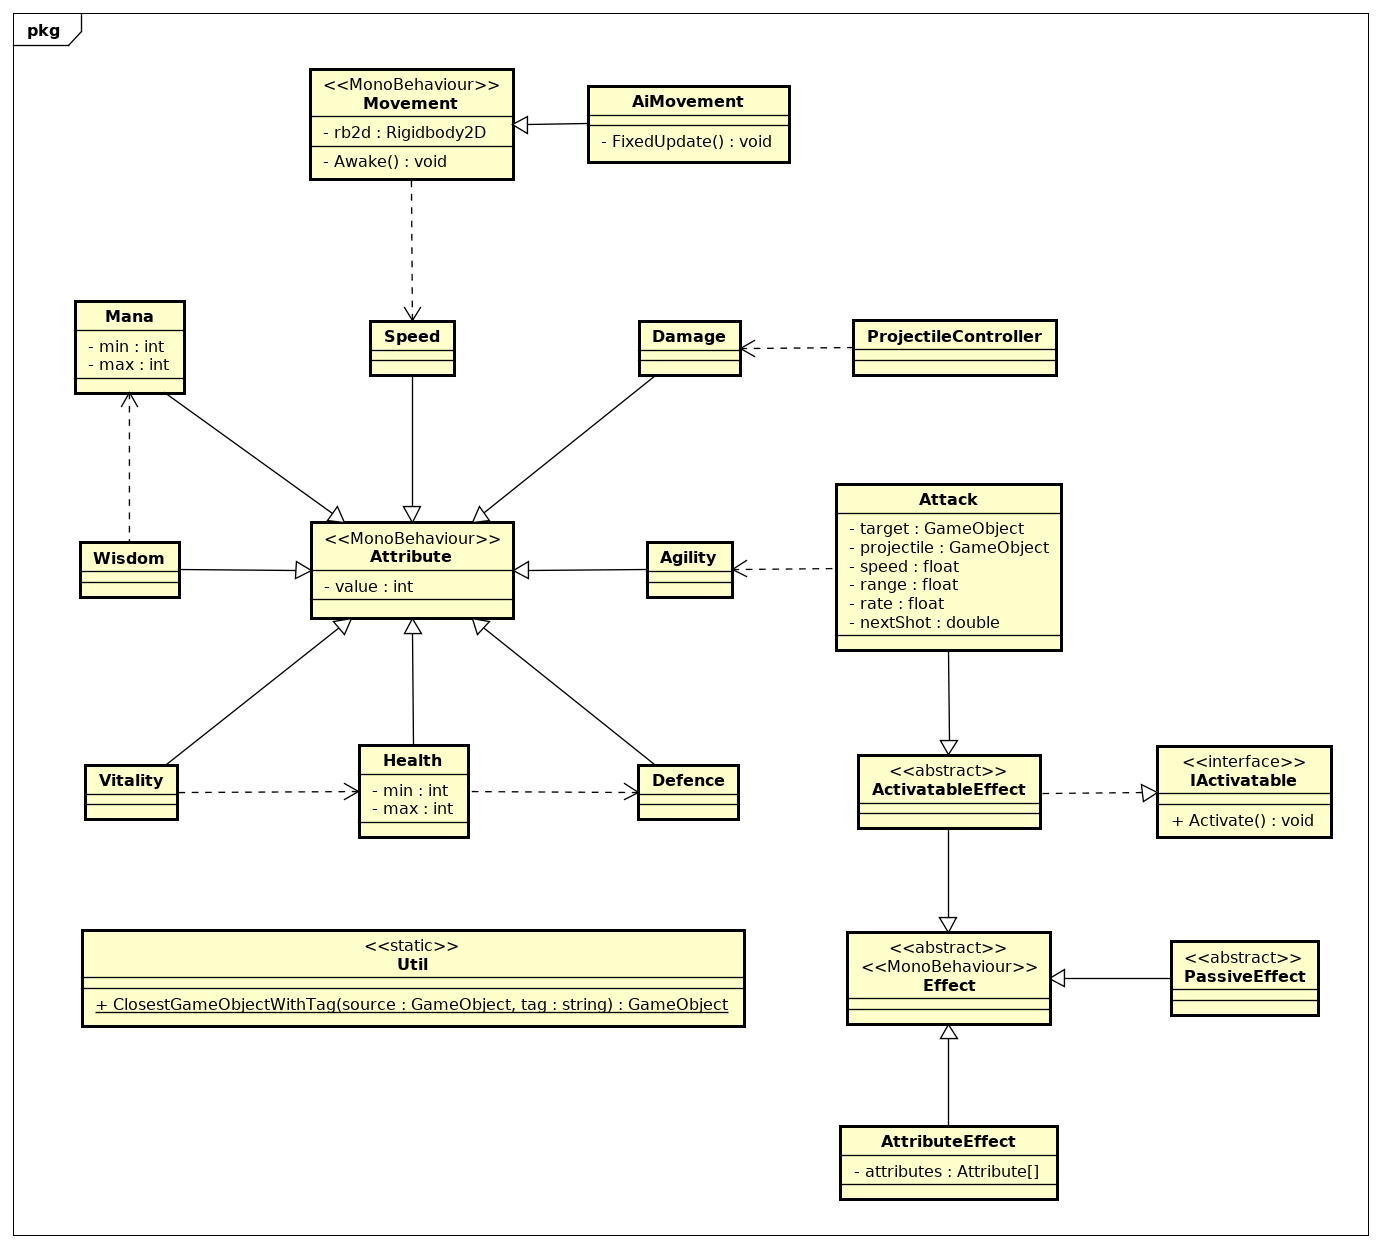
\includegraphics[width=\textwidth]{./interaction.png}
\end{center}

\begin{center}
 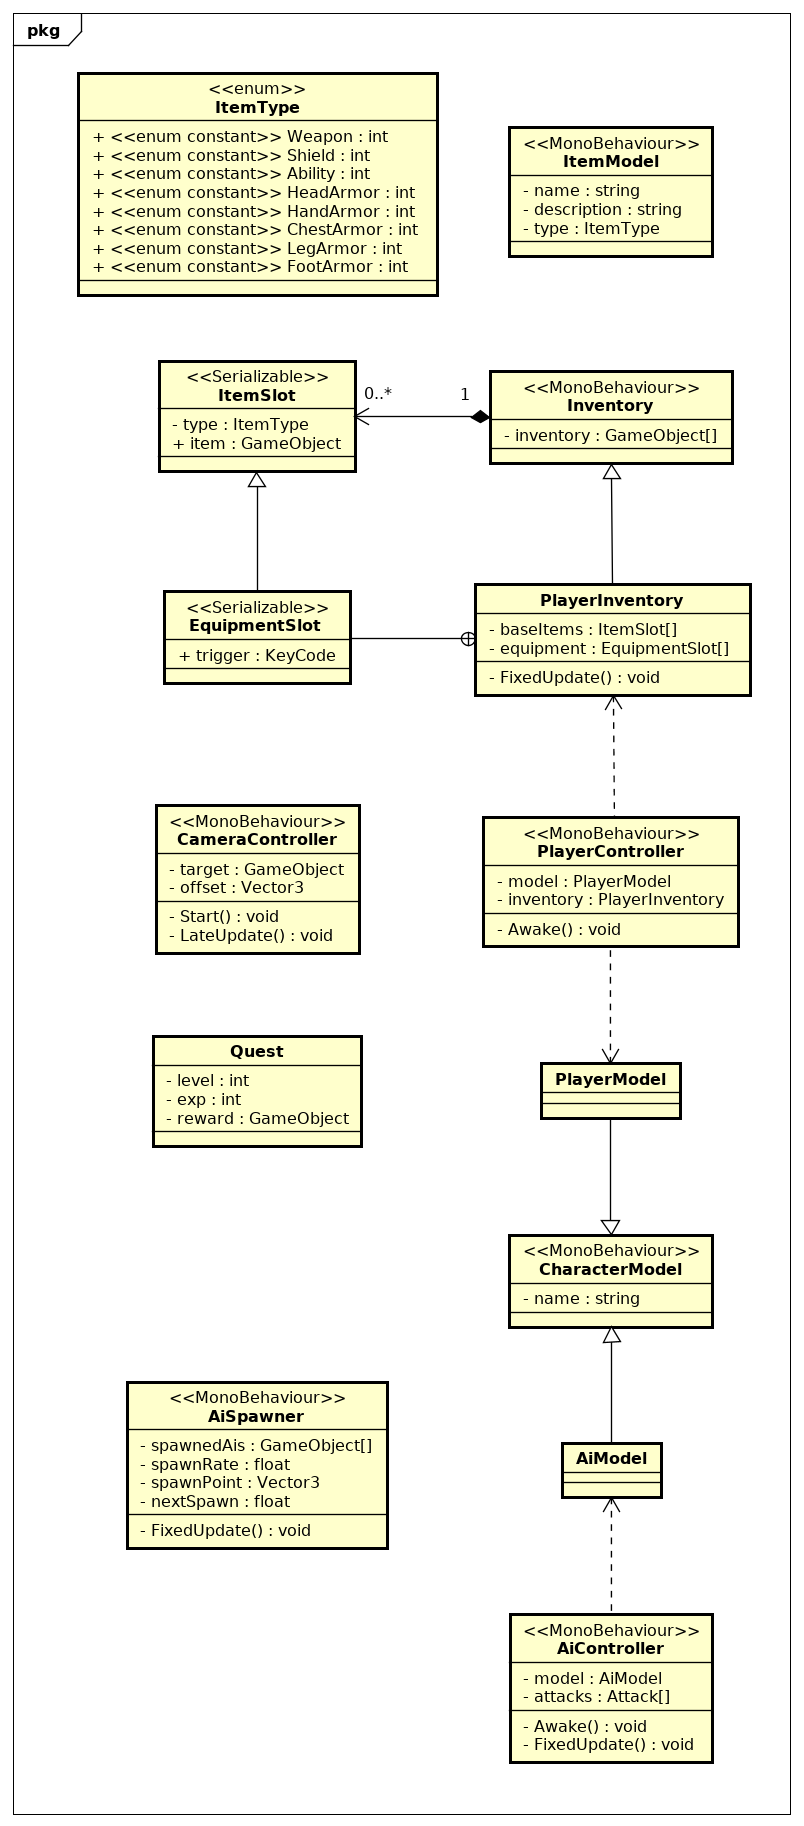
\includegraphics[height=\textheight]{./data.png}
\end{center}

\section{Implementation}
This section provides information about the development process and splits different subjects into specific units and tasks.
Multiple units are contained in a milestone.
\subsection{\texttt{/Milestone/} Basic Prototype}
A simple prototype to get into Unity and test the development environment.
\\ Due to date: \texttt{27.09.2016}
\subsection{\texttt{/Milestone/} Project Documentation}
Submission of all required documents.
\\ Due to date: \texttt{04.10.2016}
\subsubsection{\texttt{/Unit/} Project Requirements}
Definition of the project requirements.
\subsubsection{\texttt{/Unit/} Feasibility Study}
A study about the projects feasibility to check whether the project is possible and also to choose a specific path for the development process.
\subsubsection{\texttt{/Unit/} Functional Specification}
Definition of all features the project has to provide due to its date of approval.
\subsubsection{\texttt{/Unit/} Project Manual}
Start of this document.
\subsection{\texttt{/Milestone/} TDOT TGM}
A prototype for presentation to use for the open-door day at school.
\\ Due to date: \texttt{22.11.2016}
\subsection{\texttt{/Milestone/} Core}
Completion of the core.
\\ Due to date: \texttt{27.12.2016}
\subsection{\texttt{/Milestone/} Prototype}
A prototype for presentation at project approval.
\\ Due to date: \texttt{17.01.2017}
\subsection{\texttt{/Milestone/} Project Approval}
Official date of approval for the project including its presentation.
\\ Due to date: \texttt{24.01.2017}

\end{document}